\subsection{Base\-Star  Class Reference}
\label{class_basestar}\index{BaseStar@{Base\-Star}}
The base class for handling stars. Used by all matching routines. 


{\tt \#include $<$basestar.h$>$}

Inheritance diagram for Base\-Star::\begin{figure}[H]
\begin{center}
\leavevmode
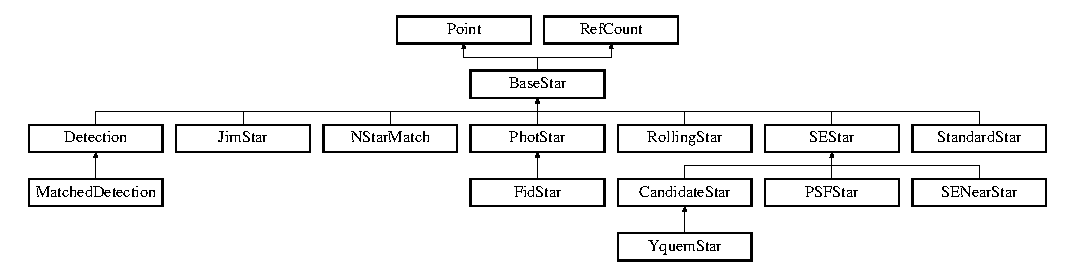
\includegraphics[height=3.27869cm]{class_basestar}
\end{center}
\end{figure}
\subsubsection*{Public Methods}
\begin{CompactItemize}
\item 
\index{BaseStar@{BaseStar}!BaseStar@{Base\-Star}}\index{BaseStar@{BaseStar}!BaseStar@{Base\-Star}}
{\bf Base\-Star} ()\label{class_basestar_a0}

\item 
\index{BaseStar@{BaseStar}!BaseStar@{Base\-Star}}\index{BaseStar@{BaseStar}!BaseStar@{Base\-Star}}
{\bf Base\-Star} (double xx, double yy, double ff)\label{class_basestar_a1}

\begin{CompactList}\small\item\em constructor.\item\end{CompactList}\item 
\index{BaseStar@{BaseStar}!BaseStar@{Base\-Star}}\index{BaseStar@{BaseStar}!BaseStar@{Base\-Star}}
{\bf Base\-Star} (const {\bf Point} \&a\_\-point, double a\_\-flux)\label{class_basestar_a2}

\item 
\index{X@{X}!BaseStar@{Base\-Star}}\index{BaseStar@{BaseStar}!X@{X}}
double {\bf X} () const\label{class_basestar_a3}

\begin{CompactList}\small\item\em access stuff.\item\end{CompactList}\item 
\index{Y@{Y}!BaseStar@{Base\-Star}}\index{BaseStar@{BaseStar}!Y@{Y}}
double {\bf Y} () const\label{class_basestar_a4}

\begin{CompactList}\small\item\em .\item\end{CompactList}\item 
\index{read_it@{read\_\-it}!BaseStar@{Base\-Star}}\index{BaseStar@{BaseStar}!read_it@{read\_\-it}}
void {\bf read\_\-it} (istream \&rd, const char $\ast$format)\label{class_basestar_a5}

\item 
\index{write@{write}!BaseStar@{Base\-Star}}\index{BaseStar@{BaseStar}!write@{write}}
virtual void {\bf write} (ostream \&s=cout) const\label{class_basestar_a6}

\item 
\index{writen@{writen}!BaseStar@{Base\-Star}}\index{BaseStar@{BaseStar}!writen@{writen}}
virtual void {\bf writen} (ostream \&s=cout) const\label{class_basestar_a7}

\item 
\index{dump@{dump}!BaseStar@{Base\-Star}}\index{BaseStar@{BaseStar}!dump@{dump}}
virtual void {\bf dump} (ostream \&stream=cout) const\label{class_basestar_a8}

\item 
\index{dumpn@{dumpn}!BaseStar@{Base\-Star}}\index{BaseStar@{BaseStar}!dumpn@{dumpn}}
virtual void {\bf dumpn} (ostream \&stream=cout) const\label{class_basestar_a9}

\item 
\index{operator=@{operator=}!BaseStar@{Base\-Star}}\index{BaseStar@{BaseStar}!operator=@{operator=}}
Base\-Star\& {\bf operator=} (const {\bf Point} \&P)\label{class_basestar_a10}

\item 
\index{~BaseStar@{$\sim$BaseStar}!BaseStar@{Base\-Star}}\index{BaseStar@{BaseStar}!~BaseStar@{$\sim$Base\-Star}}
virtual {\bf $\sim$Base\-Star} ()\label{class_basestar_a11}

\item 
\index{WriteHeader_@{WriteHeader\_\-}!BaseStar@{Base\-Star}}\index{BaseStar@{BaseStar}!WriteHeader_@{Write\-Header\_\-}}
virtual string {\bf Write\-Header\_\-} (ostream \&stream=cout, const char $\ast$i=NULL) const\label{class_basestar_a12}

\item 
\index{WriteHeader@{WriteHeader}!BaseStar@{Base\-Star}}\index{BaseStar@{BaseStar}!WriteHeader@{Write\-Header}}
virtual void {\bf Write\-Header} (ostream \&stream=cout) const\label{class_basestar_a13}

\end{CompactItemize}
\subsubsection*{Public Attributes}
\begin{CompactItemize}
\item 
\index{flux@{flux}!BaseStar@{Base\-Star}}\index{BaseStar@{BaseStar}!flux@{flux}}
double {\bf flux}\label{class_basestar_m0}

\end{CompactItemize}
\subsubsection*{Static Public Methods}
\begin{CompactItemize}
\item 
\index{read@{read}!BaseStar@{Base\-Star}}\index{BaseStar@{BaseStar}!read@{read}}
Base\-Star$\ast$ {\bf read} (istream \&rd, const char $\ast$format)\label{class_basestar_d0}

\item 
\index{TypeName@{TypeName}!BaseStar@{Base\-Star}}\index{BaseStar@{BaseStar}!TypeName@{Type\-Name}}
const char$\ast$ {\bf Type\-Name} ()\label{class_basestar_d1}

\end{CompactItemize}
\subsubsection*{Friends}
\begin{CompactItemize}
\item 
\index{operator<<@{operator$<$$<$}!BaseStar@{Base\-Star}}\index{BaseStar@{BaseStar}!operator<<@{operator$<$$<$}}
ostream\& {\bf operator$<$$<$} (ostream \&stream, const Base\-Star \&s)\label{class_basestar_l0}

\begin{CompactList}\small\item\em allows cout $<$$<$ a\-Base\-Star;.\item\end{CompactList}\end{CompactItemize}


\subsubsection{Detailed Description}
The base class for handling stars. Used by all matching routines.



The documentation for this class was generated from the following file:\begin{CompactItemize}
\item 
{\bf basestar.h}\end{CompactItemize}
